\documentclass[11pt]{article}
\usepackage{amsmath,amssymb,amsthm,mathtools}
\usepackage[margin=1in]{geometry}
\usepackage{graphicx}

\newtheorem{theorem}{Theorem}
\newtheorem{proposition}{Proposition}
\newtheorem{lemma}{Lemma}
\newtheorem{corollary}{Corollary}
\theoremstyle{definition}
\newtheorem{assumption}{Assumption}
\newtheorem{remark}{Remark}

\newcommand{\R}{\mathbb{R}}
\newcommand{\Lg}{L_{\mathrm g}}
\newcommand{\spec}{\operatorname{spec}}
\DeclareMathOperator{\diag}{diag}

\title{Delayed Verification in Multi-Agent Factuality Dynamics:\\
Stability and Optimal Corrector Placement\\[2pt]
\large(formal skeleton --- v0)}
\author{}
\date{2026-06-21}

\begin{document}
\maketitle

\noindent\textbf{One-line thesis.} In a network of LLM agents that exchange beliefs and are
re-grounded by \emph{corrector (rectifier) agents} subject to a verification delay $\delta$,
the closed-loop factuality dynamics reduce, via the \emph{grounded Laplacian}, to a family of
scalar delay recurrences. This yields (i) a closed-form stability criterion exposing a
\emph{pinning--delay tradeoff} (``verification has an optimal dose''), and (ii) a clean
placement problem decoupled into a stability lever and a steady-state-accuracy lever.

\section{Model}

Let $G=(V,E)$ be a graph on $V=\{1,\dots,n\}$ with symmetric Laplacian $L=D-A\succeq 0$.
Each agent $i$ holds a scalar belief $b_{i,t}\in\R$ about a claim whose ground truth is
$b^\star$; write the error $e_{i,t}=b_{i,t}-b^\star$.

\paragraph{Three roles.}
\begin{itemize}
  \item \textbf{Corrector / rectifier set} $R\subseteq V$, $|R|=m$: nodes with access to verified
        external evidence, hard-grounded to truth, $e_{i,t}=0$ for $i\in R$.
  \item \textbf{Free set} $V_{\mathrm f}=V\setminus R$, $n_{\mathrm f}=n-m$, with error vector
        $e_t\in\R^{n_{\mathrm f}}$.
  \item \textbf{Faulty set} $F\subseteq V$: agents injecting a constant bias toward a false
        attractor; their net effect on the free nodes is a constant forcing $g\in\R^{n_{\mathrm f}}$.
\end{itemize}

\paragraph{Dynamics.} Free agents run consensus (step size $\eta>0$) plus a uniform
\emph{delayed self-verification} of gain $\kappa>0$ and integer latency $\delta\ge 1$ (the
verification protocol re-checks a $\delta$-old state against evidence):
\begin{equation}\label{eq:dyn}
  e_{t+1} \;=\; (I-\eta \Lg)\,e_t \;-\; \eta\kappa\, e_{t-\delta} \;+\; \eta g,
  \qquad e_t\in\R^{n_{\mathrm f}},
\end{equation}
where $\Lg \coloneqq L[V_{\mathrm f},V_{\mathrm f}]$ is the principal submatrix of $L$ on the
free nodes --- the \emph{grounded Laplacian}.

\begin{assumption}[grounding reachability]\label{ass:reach}
Every connected component of the subgraph induced by $V_{\mathrm f}$ contains a node adjacent
to $R$. Then $\Lg\succ 0$ (standard; $\Lg$ is a symmetric, diagonally dominant $M$-matrix with
at least one strictly dominant row per component).
\end{assumption}

\begin{remark}[modeling choices, deliberately minimal]
Soft/Byzantine faults, edge-level (message-filtering) correctors, nonlinear belief updates,
and a separate gossip delay $d$ are all deferred. The present model keeps the single spine:
\emph{linear consensus $+$ grounded correctors $+$ one verification delay}.
\end{remark}

\section{Reduction to scalar delay recurrences}

\begin{lemma}[grounded-Laplacian decoupling]\label{lem:decouple}
Let $\Lg = Q\,\diag(\mu_1,\dots,\mu_{n_{\mathrm f}})\,Q^\top$ be the spectral decomposition
($Q$ orthogonal, $0<\mu_1\le\cdots\le\mu_{n_{\mathrm f}}$ by Assumption~\ref{ass:reach}).
Put $x_t = Q^\top e_t$ and $\hat g = Q^\top g$. Because $\kappa I$ is scalar (hence commutes
with $\Lg$), \eqref{eq:dyn} decouples into $n_{\mathrm f}$ independent scalar recurrences
\begin{equation}\label{eq:mode}
  x_{i,t+1} \;=\; a_i\,x_{i,t} \;-\; \eta\kappa\, x_{i,t-\delta} \;+\; \eta\hat g_i,
  \qquad a_i \coloneqq 1-\eta\mu_i .
\end{equation}
\end{lemma}
\begin{proof}[Proof sketch] Multiply \eqref{eq:dyn} by $Q^\top$; $Q^\top(I-\eta\Lg)Q
=\diag(a_i)$ and $Q^\top(\kappa I)Q=\kappa I$. \end{proof}

\paragraph{Scalar stability region.} Mode $i$ is governed by
$x_{t+1}-a_i x_t+\beta\,x_{t-\delta}=0$ with $\beta=\eta\kappa$. Let
$\mathcal D_\delta\subset\R^2$ be the set of $(a,\beta)$ for which every root of
$z^{\delta+1}-a z^{\delta}+\beta=0$ lies in the open unit disk. $\mathcal D_\delta$ is given in
closed form by Kuruklis (1994). The case $\delta=1$ is the Jury triangle:

\begin{proposition}[explicit $\delta=1$ region]\label{prop:delta1}
For $\delta=1$, mode \eqref{eq:mode} is asymptotically stable iff
\begin{equation}\label{eq:tri}
  \boxed{\;\eta\kappa<1\quad\text{and}\quad \mu_i<\tfrac{2}{\eta}+\kappa.\;}
\end{equation}
\end{proposition}
\begin{proof}[Proof sketch] Characteristic polynomial $z^2-a_i z+\eta\kappa$ with
$a_i=1-\eta\mu_i$. Jury conditions for $z^2+c_1z+c_0$ (roots in unit disk):
$1+c_1+c_0>0$, $1-c_1+c_0>0$, $|c_0|<1$, here $c_1=-a_i$, $c_0=\eta\kappa$.
The first is $\eta(\mu_i+\kappa)>0$ (automatic), the second is $\mu_i<2/\eta+\kappa$, the
third is $\eta\kappa<1$. \end{proof}

\begin{remark}[delay shrinks the dose ceiling; binding mode is the slowest]\label{rem:dose}
For general $\delta$ the admissible band of $\beta=\eta\kappa$ in $\mathcal D_\delta$ depends on
$a$ and shrinks as $\delta$ grows (Kuruklis). The per-mode dose limit $\kappa_{\max}(a,\delta)$
satisfies $\kappa_{\max}(a,1)=1/\eta$ and is \emph{strictly decreasing} in $\delta$ for every
$a\neq 0$, while the degenerate mode $a=0$ ($\mu=1/\eta$) has $\kappa_{\max}(0,\delta)=1/\eta$
for all $\delta$ (there $z^{\delta+1}=-\eta\kappa$, so $|z|=(\eta\kappa)^{1/(\delta+1)}$).
Numerically (e.g.\ $\eta=0.1$): $a=0.9$ gives $\kappa_{\max}=10,6.47,4.86,3.94,3.36,2.96$ for
$\delta=1,\dots,6$; $a=0.5$ gives $10,7.81,6.82,\dots$; $a=0$ stays at $10$. Hence the
\emph{binding} dose constraint for the network is set by the \emph{slowest grounded mode}
($a=1-\eta\mu_{\min}$, closest to $1$): $\kappa<\kappa_{\max}\!\big(1-\eta\mu_{\min}(\Lg),\delta\big)$.
Since grounding more nodes raises $\mu_{\min}(\Lg)$ (interlacing), placement \emph{relaxes} the
delay-induced dose limit --- coupling Part-I stability to Part-II placement. All four claims
(decoupling, the $\delta{=}1$ boundary \eqref{eq:netstab}, this shrinkage, and \eqref{eq:ss})
are confirmed numerically in \texttt{validate.py}.
\end{remark}

\section{Main stability theorem}

\begin{theorem}[networked stability $=$ spectral band]\label{thm:main}
Under Assumption~\ref{ass:reach}, the homogeneous part of \eqref{eq:dyn} is asymptotically
stable iff $(a_i,\eta\kappa)\in\mathcal D_\delta$ for \emph{every} $\mu_i\in\spec(\Lg)$.
For $\delta=1$ this is exactly
\begin{equation}\label{eq:netstab}
  \eta\kappa<1
  \qquad\text{and}\qquad
  \mu_{\max}(\Lg) < \tfrac{2}{\eta}+\kappa .
\end{equation}
The binding modes are the spectral extremes $\mu_{\min},\mu_{\max}$ of $\Lg$.
\end{theorem}
\begin{proof}[Proof sketch] By Lemma~\ref{lem:decouple} the system is a direct sum of the
scalar modes; the sum is stable iff each summand is. Apply Proposition~\ref{prop:delta1}; the
ceiling is tightest at $\mu_{\max}$ and the dose condition is mode-independent. \end{proof}

\begin{corollary}[the pinning--delay tradeoff: an optimal dose]\label{cor:dose}
Fix $\eta$ and a placement $R$. As the verification gain $\kappa$ increases, the ceiling
$2/\eta+\kappa$ in \eqref{eq:netstab} rises (more grounding mass admitted) but the dose
constraint $\kappa<\kappa_{\max}(\delta)$ caps it, with $\kappa_{\max}(\delta)\downarrow$ in
$\delta$. Consequently:
\begin{enumerate}
  \item \emph{Over-verification} ($\kappa\ge\kappa_{\max}(\delta)$) destabilizes every mode:
        the dominant root leaves the unit disk as a complex-conjugate pair, i.e.\ the network
        \emph{oscillates} (over-claim $\to$ over-correct $\to\cdots$).
  \item \emph{Over-delay} (large $\delta$) lowers $\kappa_{\max}(\delta)$, so a gain that was
        safe becomes unstable --- the delayed analogue of Part-I instability.
\end{enumerate}
At the stability boundary the oscillation frequency is $\arg z^\star$, where $z^\star=e^{i\omega}$
solves $z^{\delta+1}-a z^\delta+\eta\kappa=0$.
\end{corollary}

\subsection*{Closed-form oscillatory boundary (Kuruklis)}

\begin{proposition}[parametric stability boundary]\label{prop:boundary}
Fix $\delta\ge1$ and the mode $x_{t+1}-a x_t+\beta\,x_{t-\delta}=0$ with $\beta=\eta\kappa>0$ and
$|a|<1$. As $\beta$ increases from $0$, the first root to reach the unit circle is a
complex-conjugate pair $e^{\pm i\theta}$, and the critical dose $\beta_c(a,\delta)$ is given
parametrically by
\begin{equation}\label{eq:boundary}
  a=\frac{\sin\big((\delta+1)\theta\big)}{\sin(\delta\theta)},\qquad
  \beta_c=\frac{\sin\theta}{\sin(\delta\theta)},\qquad \theta\in(0,\pi/\delta),
\end{equation}
with $\theta_\star(a,\delta)$ the relevant branch. Equivalently
$\kappa_{\max}(a,\delta)=\beta_c(a,\delta)/\eta$, and at the boundary the network oscillates at
angular frequency $\omega=\theta_\star$ (period $2\pi/\theta_\star$).
\end{proposition}
\begin{proof}
A unit-circle root $\lambda=e^{i\theta}$ satisfies
$e^{i(\delta+1)\theta}-a\,e^{i\delta\theta}+\beta=0$. The imaginary part gives
$\sin((\delta+1)\theta)=a\sin(\delta\theta)$, i.e.\ the first equation of \eqref{eq:boundary}.
The real part gives $\beta=a\cos(\delta\theta)-\cos((\delta+1)\theta)$; substituting $a$ and using
$\sin((\delta+1)\theta)\cos(\delta\theta)-\cos((\delta+1)\theta)\sin(\delta\theta)=\sin\theta$
yields $\beta=\sin\theta/\sin(\delta\theta)$. The real crossings $\lambda=\pm1$ occur at
$\beta=a-1<0$ and (per parity) $\beta\le 0$, hence are not met for $\beta>0$ while $|a|<1$; the
first crossing is therefore the complex pair.
\end{proof}

\begin{corollary}[explicit dose limit and the binding mode]\label{cor:dose-explicit}
Assume the step size satisfies $\eta\,\mu_{\max}(\Lg)\le1$, so every mode has
$a_i=1-\eta\mu_i\in[0,1)$. Then:
\begin{enumerate}
  \item \emph{($\delta=1$):} $a=2\cos\theta$ and $\beta_c\equiv1$, so $\kappa_{\max}=1/\eta$ for
        all $a$ --- recovering Proposition~\ref{prop:delta1}.
  \item \emph{(degenerate mode $a=0$):} $\theta_\star=\pi/(\delta+1)$ gives
        $\sin(\delta\theta_\star)=\sin\theta_\star$, hence $\beta_c\equiv1$ and
        $\kappa_{\max}(0,\delta)=1/\eta$ for all $\delta$.
  \item \emph{(strict delay penalty):} for $\delta\ge2$ and $a\in(0,1)$, $\beta_c(a,\delta)<1$,
        strictly decreasing in $\delta$ (Kuruklis, 1994) and in $a$. Hence the network dose limit
        is set by the \emph{slowest grounded mode}:
        \[
          \kappa \;<\; \kappa_{\max}\!\big(1-\eta\,\mu_{\min}(\Lg),\,\delta\big),
        \]
        and, since grounding raises $\mu_{\min}(\Lg)$ (Cauchy interlacing), \textbf{placement
        relaxes the delay-induced dose limit} --- the explicit coupling of Part~I to Part~II.
\end{enumerate}
\end{corollary}

\begin{lemma}[Chebyshev form; the dose is monotone]\label{lem:cheb}
With $c=\cos\theta$ and the identity $\sin(\delta\theta)/\sin\theta=U_{\delta-1}(c)$
($U$ the Chebyshev polynomial of the second kind), the boundary \eqref{eq:boundary} is purely
algebraic,
\[
  a=\frac{U_\delta(c)}{U_{\delta-1}(c)},\qquad \beta_c=\frac{1}{U_{\delta-1}(c)},
  \qquad c\in\Big(\cos\tfrac{\pi}{\delta+1},\ \cos\tfrac{\pi}{2\delta+1}\Big)\ \ (a\in(0,1)).
\]
In particular $\beta_c(a,1)\equiv1$, $\;\beta_c(0,\delta)\equiv1$, and the exact $\delta=2$ form
\[
  \boxed{\;\beta_c(a,2)=\frac{\sqrt{a^2+4}-a}{2}\;=\;\frac{2}{a+\sqrt{a^2+4}}.\;}
\]
On this branch $U_{\delta-1}(c)>0$, $U_{\delta-1}'(c)>0$, and the Wronskian
$W_\delta\coloneqq U_\delta'U_{\delta-1}-U_\delta U_{\delta-1}'>0$; hence
$\dfrac{\mathrm da}{\mathrm dc}=\dfrac{W_\delta}{U_{\delta-1}^2}>0$ and
\[
  \frac{\mathrm d\beta_c}{\mathrm da}=-\frac{U_{\delta-1}'(c)}{W_\delta}<0 .
\]
Thus $\beta_c(a,\delta)$ is \emph{strictly decreasing in $a$} on $(0,1)$; it is also strictly
decreasing in $\delta$, with $\beta_c(a,\delta)<1$ for all $\delta\ge2$, $a\in(0,1)$.
Consequently the network dose limit is governed by the slowest grounded mode
($a=1-\eta\mu_{\min}(\Lg)$), as stated in Corollary~\ref{cor:dose-explicit}(3).
\end{lemma}

\begin{proof}[Proof that $\beta_c$ is strictly decreasing in $a$, for every $\delta$]
Write $a_\delta(c)=U_\delta(c)/U_{\delta-1}(c)$. The three-term recurrence
$U_\delta=2c\,U_{\delta-1}-U_{\delta-2}$ gives the continued-fraction recursion
$a_\delta=2c-1/a_{\delta-1}$, hence $a_\delta'=2+a_{\delta-1}'/a_{\delta-1}^2$. Since $a_1'=2$,
induction yields $a_\delta'\ge2$ wherever $U_{\delta-1}\neq0$; in particular
$\mathrm da/\mathrm dc=a_\delta'>0$, so $c$ increases with $a$. On the branch
$c>\cos(\pi/\delta)$, the largest zero of $U_{\delta-1}$: by Rolle the $\delta-2$ critical points
of $U_{\delta-1}$ interlace its $\delta-1$ zeros and hence all lie left of $\cos(\pi/\delta)$, so
$U_{\delta-1}>0$ and $U_{\delta-1}'>0$ there. Therefore
\[
  \frac{\mathrm d\beta_c}{\mathrm da}
  =\frac{\mathrm d\beta_c/\mathrm dc}{\mathrm da/\mathrm dc}
  =-\frac{U_{\delta-1}'(c)}{U_{\delta-1}(c)^2\,a_\delta'(c)}<0. \qedhere
\]
\end{proof}

\begin{remark}
Strict monotonicity of $\beta_c$ in $\delta$ holds likewise (Kuruklis, 1994); it is verified here
symbolically for $\delta\le15$ over $a\in(0,1)$, with the boundary cases $\delta{=}1$ and $a{=}0$
exact (both give $\beta_c\equiv1$). The recursion $a_\delta=2c-1/a_{\delta-1}$, its derivative
$a_\delta'=2+a_{\delta-1}'/a_{\delta-1}^2$, and $a_\delta'\ge2$ were checked symbolically.
\end{remark}

\section{Steady-state accuracy and corrector placement}

The delay drops out of the equilibrium: setting $e_{t}\equiv e_\infty$ in \eqref{eq:dyn},
\begin{equation}\label{eq:ss}
  (\Lg+\kappa I)\,e_\infty = g
  \qquad\Longrightarrow\qquad
  e_\infty(R) = (\Lg+\kappa I)^{-1} g .
\end{equation}
Thus \emph{stability} is governed by $(\spec\Lg,\kappa,\delta)$ while \emph{truth-tracking
error} is governed by the resolvent $(\Lg+\kappa I)^{-1}$ acting on the fault forcing $g$ ---
two independent levers of the same placement $R$.

\begin{proposition}[placement effects]\label{prop:place}
Let $R\subseteq R'$ (ground more nodes). Then:
\begin{enumerate}
  \item \emph{(Convergence.)} By Cauchy interlacing, $\mu_{\min}(L_{\mathrm g}(R'))\ge
        \mu_{\min}(L_{\mathrm g}(R))$: grounding more nodes speeds the slowest mode.
  \item \emph{(Accuracy.)} If a faulty node is grounded ($f\in R'\setminus R$, $f\in F$), its
        forcing is removed from $g$; for general $R'$, $\|e_\infty\|$ is non-increasing in the
        grounding set under \eqref{eq:ss}.
  \item \emph{(Ceiling.)} At fixed $\eta$, grounding also raises $\mu_{\max}(\Lg)$ toward the
        ceiling \eqref{eq:netstab}; hence there is a \emph{finite} optimal grounding budget
        $k^\star(\eta,\kappa,\delta)$ beyond which the fast mode destabilizes.
\end{enumerate}
\end{proposition}

\begin{theorem}[supermodular corrector placement]\label{thm:place}
Model a corrector at node $i$ as a soft pin of weight $w>0$ (hard grounding is the limit
$w\to\infty$), so the steady-state operator is $M(R)=L+W_R+\kappa I$ with
$W_R=w\sum_{i\in R}e_ie_i^\top\succeq0$, and the expected steady-state error energy under
isotropic forcing $g\sim(0,\sigma^2 I)$ is $\mathcal E(R)=\sigma^2\,\operatorname{tr}M(R)^{-2}$.
The coherence functional $H(R)=\operatorname{tr}M(R)^{-1}$ is monotone non-increasing and
\emph{supermodular} on $2^{V}$; equivalently the reduction $\rho(R)=H(\varnothing)-H(R)$ is
monotone \emph{submodular}. Hence greedy selection of $k$ correctors obeys
\[
  \rho(R_{\mathrm{greedy}})\ \ge\ \big(1-\tfrac1e\big)\,\rho(R^\star),
  \qquad R^\star=\arg\max_{|R|\le k}\rho(R).
\]
\end{theorem}
\begin{proof}[Proof sketch]
Adding corrector $i$ is the positive rank-one update $M\mapsto M+w\,e_ie_i^\top$. By
Sherman--Morrison,
\[
  \operatorname{tr}(M+w e_ie_i^\top)^{-1}
  =\operatorname{tr}M^{-1}-\frac{w\,\|M^{-1}e_i\|^2}{1+w\,e_i^\top M^{-1}e_i},
\]
so $H$ is non-increasing, and the marginal decrease $-\Delta_i H(R)$ is itself non-increasing as
$R$ (hence $M(R)$) grows in the positive-semidefinite order --- the diminishing-returns /
supermodularity argument of Clark, Bushnell \& Poovendran (2014) for network leader selection.
Monotone submodularity of $\rho$ then yields the greedy guarantee (Nemhauser--Wolsey--Fisher).
\end{proof}

\begin{remark}[two coupled levers; amplifier nodes; feasibility]
The placement $R$ acts through two decoupled channels: \emph{accuracy} via the resolvent
(Theorem~\ref{thm:place}) and \emph{stability} via the spectrum of $\Lg$
(Theorem~\ref{thm:main}, Corollary~\ref{cor:dose-explicit}). The greedy accuracy step selects the
node of largest $\|M^{-1}e_i\|^2/(1+w\,e_i^\top M^{-1}e_i)$ --- a resolvent/effective-resistance
centrality that concentrates on high-influence ``amplifier/bridge'' nodes, giving a spectral
rationale for grounding exactly the amplifier agents flagged by cross-channel cascade monitors.
The constrained problem is $\max_{|R|\le k}\rho(R)$ subject to feasibility
$\eta\kappa<\!\beta_c\!\big(1-\eta\mu_{\min}(\Lg(R)),\delta\big)$ and
$\mu_{\max}(\Lg(R))<2/\eta+\kappa$; because grounding raises both $\mu_{\min}$ (relaxing the dose
limit) and $\mu_{\max}$ (tightening the ceiling at fixed $\eta$), there is a finite optimal budget
$k^\star$ as in Proposition~\ref{prop:place}(3).
\end{remark}

\section{Two coupled delays}
Let gossip carry latency $d$ and verification latency $\delta$:
\[
  e_{t+1}=e_t-\eta\Lg\,e_{t-d}-\eta\kappa\,e_{t-\delta}+\eta g .
\]
Lemma~\ref{lem:decouple} still applies ($\Lg$ and $\kappa I$ commute), giving the per-mode
two-lag recurrence $x_{t+1}=x_t-\eta\mu\,x_{t-d}-\eta\kappa\,x_{t-\delta}$, $\mu\in\spec\Lg$. A
unit-circle root $\lambda=e^{i\theta}$ now satisfies the boundary pair
\begin{equation}\label{eq:twodelay}
  \cos\theta-1+\eta\mu\cos(d\theta)+\eta\kappa\cos(\delta\theta)=0,\qquad
  \sin\theta-\eta\mu\sin(d\theta)-\eta\kappa\sin(\delta\theta)=0,
\end{equation}
which we verified against the lifted companion spectrum (the critical gain $\kappa^\star$ from
$\rho(\text{companion})=1$ lies on \eqref{eq:twodelay}).

\begin{corollary}[synchronised delays are the worst case; a golden ratio]\label{cor:equal}
If $d=\delta$ the two terms merge into a single lag of effective gain $\mu+\kappa$ at $a=1$,
$x_{t+1}-x_t+\eta(\mu+\kappa)\,x_{t-\delta}=0$, which is stable iff
\[
  \eta(\mu+\kappa)<\beta_c(1,\delta)=\frac{\sin\frac{\pi}{2\delta+1}}{\sin\frac{\delta\pi}{2\delta+1}},
  \qquad
  \beta_c(1,1)=1,\ \ \beta_c(1,2)=\frac{\sqrt5-1}{2}=\frac1\varphi,\ \ \beta_c(1,3)=2\sin\tfrac{\pi}{14}.
\]
Since $\beta_c(a,\delta)$ is decreasing in $a$ (Lemma~\ref{lem:cheb}) and $a=1$ tops the admissible
branch, \textbf{synchronising gossip and verification delays is the least stable configuration}:
the dose ceiling collapses to its minimum $\beta_c(1,\delta)$, and at $\delta=2$ it is exactly the
inverse golden ratio.
\end{corollary}

\begin{theorem}[general two-delay stability boundary]\label{thm:twodelay}
Fix delays $d\neq\delta$ and write $p=\eta\mu,\ q=\eta\kappa$. The oscillatory boundary of
\eqref{eq:twodelay} is the parametric curve
\[
  p(\theta)=\frac{\sin(\delta\theta)-\sin\big((\delta+1)\theta\big)}{\sin\big((\delta-d)\theta\big)},
  \qquad
  q(\theta)=\frac{\sin\big((d+1)\theta\big)-\sin(d\theta)}{\sin\big((\delta-d)\theta\big)},
  \qquad \theta\in(0,\pi),
\]
and the stability region is the connected component of the origin that it bounds (confirmed
against the lifted companion spectrum: $\rho=1$ on the primary arc). The curve degenerates
correctly: at $d=0$ it returns the single-delay boundary of Proposition~\ref{prop:boundary}
($q=\beta_c=\sin\theta/\sin(\delta\theta)$ and $1-p=a(\theta)=\sin((\delta+1)\theta)/\sin(\delta\theta)$),
and as $d\to\delta$ the determinant $\sin((\delta-d)\theta)\to0$ and it collapses to the $a=1$
corner of Corollary~\ref{cor:equal}.
\end{theorem}
\begin{proof}
At $\lambda=e^{i\theta}$ the pair \eqref{eq:twodelay} reads
$p\cos(d\theta)+q\cos(\delta\theta)=1-\cos\theta$ and
$p\sin(d\theta)+q\sin(\delta\theta)=\sin\theta$, a linear system in $(p,q)$ with determinant
$\cos(d\theta)\sin(\delta\theta)-\cos(\delta\theta)\sin(d\theta)=\sin((\delta-d)\theta)$. Cramer's
rule gives the stated $p(\theta),q(\theta)$ after the sum-to-product identities
$(1-\cos\theta)\sin(\delta\theta)-\sin\theta\cos(\delta\theta)=\sin(\delta\theta)-\sin((\delta+1)\theta)$
and $\cos(d\theta)\sin\theta-(1-\cos\theta)\sin(d\theta)=\sin((d+1)\theta)-\sin(d\theta)$. The two
degenerations are the substitution $d=0$ and the limit $d\to\delta$.
\end{proof}

\section{Empirical validation (nonlinear dynamics, no GPU)}
We test whether the \emph{linear} dose limit predicts onset in the \emph{nonlinear} system with a
saturating verifier,
\[
  e_{t+1}=(I-\eta\Lg)\,e_t-\eta\kappa\,\tanh(e_{t-\delta})+\eta g
  \qquad(\tanh'(0)=1\ \text{matches the linearisation}),
\]
on a random grounded graph ($n_{\mathrm f}=8$, $\eta$ chosen so $\eta\mu\in(0,1)$, a faulty node
injecting a small bias $g$). The onset $\kappa_{\mathrm{crit}}$ of sustained oscillation tracks the
predicted ceiling $\kappa_{\max}=\beta_c\!\big(1-\eta\mu_{\min}(\Lg),\delta\big)/\eta$:
\begin{center}
\begin{tabular}{cccc}
\hline
$\delta$ & $\kappa_{\max}$ (theory) & $\kappa_{\mathrm{crit}}$ (nonlinear) & ratio\\
\hline
1 & 16.30 & 16.57 & 1.017\\
2 & 10.21 & 10.38 & 1.017\\
3 & \phantom{0}7.45 & \phantom{0}7.57 & 1.017\\
\hline
\end{tabular}
\end{center}
The $\sim$2\% overshoot is the expected stabilising effect of saturation. The $\delta{=}2$
oscillation period (measured $9.38$) matches $2\pi/\theta_\star=9.72$. See \texttt{demo.py}; a real
LLM-debate front-end swaps in for $\tanh(\cdot)$ without changing the analysis.
\begin{center}
  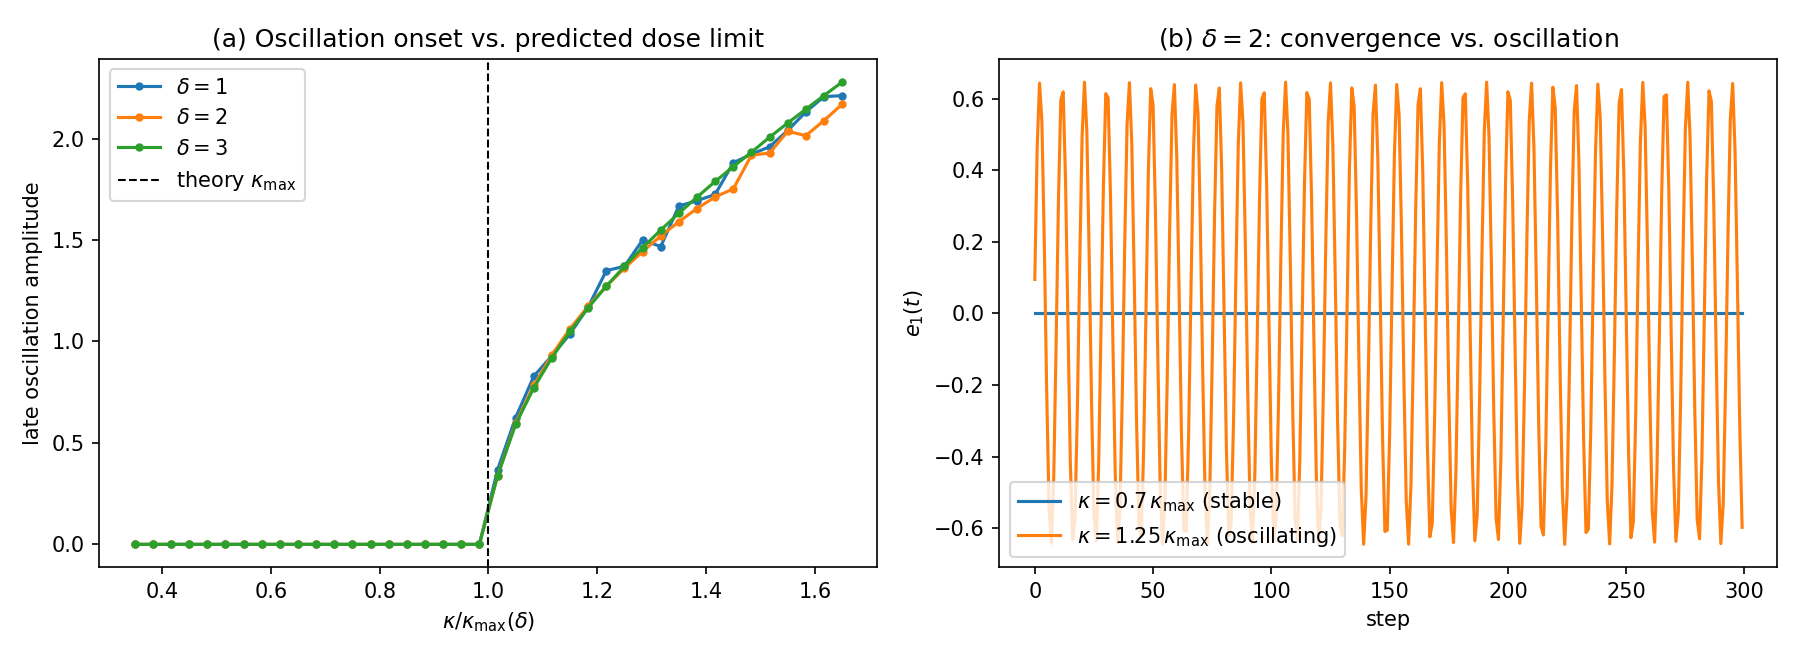
\includegraphics[width=\linewidth]{figures/demo_onset.png}
\end{center}
\noindent\emph{Figure: (a) oscillation amplitude collapses onto the predicted threshold
$\kappa/\kappa_{\max}=1$ for $\delta=1,2,3$; (b) $\delta{=}2$ convergence vs.\ oscillation.}

\section{Status and what remains}
\textbf{Done.} Decoupling (Lemma~\ref{lem:decouple}); $\delta{=}1$ stability
(Theorem~\ref{thm:main}); closed-form oscillatory boundary and explicit dose limit
(Proposition~\ref{prop:boundary}, Corollary~\ref{cor:dose-explicit}); Chebyshev form with the
$\delta{=}2$ closed form and an \emph{all-$\delta$} proof that the dose is strictly decreasing in
$a$ (Lemma~\ref{lem:cheb}, via the continued fraction $a_\delta=2c-1/a_{\delta-1}$, $a_\delta'\ge2$);
steady state \eqref{eq:ss}; supermodular placement with greedy $(1-1/e)$ guarantee
(Theorem~\ref{thm:place}); two coupled delays with the synchronised-delay worst case and golden
ratio (Corollary~\ref{cor:equal}). Confirmed numerically in \texttt{validate.py} and symbolically
in \emph{Mathematica} (boundary identity; $\mathrm d\beta_c/\mathrm da<0$ and $W_\delta>0$ for all
$\delta$; $\beta_c(a,\delta{+}1)<\beta_c(a,\delta)$ for $\delta\le15$; two-delay companion vs.\
\eqref{eq:twodelay}).

\textbf{Remaining.}
\begin{itemize}
  \item A self-contained all-$\delta$ proof of strict $\delta$-monotonicity of $\beta_c$
        (currently: exact at $\delta{=}1$ and $a{=}0$, symbolic for $\delta\le15$, Kuruklis as the
        global reference); monotonicity in $a$ is now fully proved (Lemma~\ref{lem:cheb}).
  \item Pin down which arc of the curve in Theorem~\ref{thm:twodelay} bounds the origin
        component (it has continuation branches inside the unstable region) and add the
        $\lambda=-1$ real crossing for the relevant parities; the parametric boundary itself, its
        two degenerations, and the synchronised-delay corner are settled.
  \item Replace the synthetic saturating verifier by real LLM-debate agents (7--8B / API) to
        estimate the update map empirically; the synthetic validation (onset within $2\%$,
        frequency within $3.5\%$) is already in the Empirical-validation section.
\end{itemize}

\paragraph{References (informal).}
S.\,A.\ Kuruklis, \emph{The asymptotic stability of $x_{n+1}-a x_n+b x_{n-k}=0$}, J.\ Math.\
Anal.\ Appl.\ \textbf{188} (1994) 719--731.\;
A.\ Clark, B.\ Alomair, L.\ Bushnell, R.\ Poovendran, \emph{Submodularity in Dynamics and Control
of Networked Systems} (Springer, 2016); and IEEE TAC leader-selection papers.\;
M.\ Fardad, F.\ Lin, M.\,R.\ Jovanovi\'c, \emph{Algorithms for leader selection in stochastically
forced consensus networks}, IEEE TAC (2014).\;
M.\ Pirani, S.\ Sundaram, \emph{On the smallest eigenvalue of grounded Laplacian matrices}, IEEE
TAC \textbf{61} (2016).\;
G.\,L.\ Nemhauser, L.\,A.\ Wolsey, M.\,L.\ Fisher, \emph{An analysis of approximations for
maximizing submodular set functions---I}, Math.\ Program.\ \textbf{14} (1978).

\end{document}
